\SetBgScale{1}
\SetBgAngle{0}
\SetBgOpacity{1}
\SetBgColor{white}
\SetBgHshift{0cm}
\SetBgVshift{0cm}
\SetBgContents{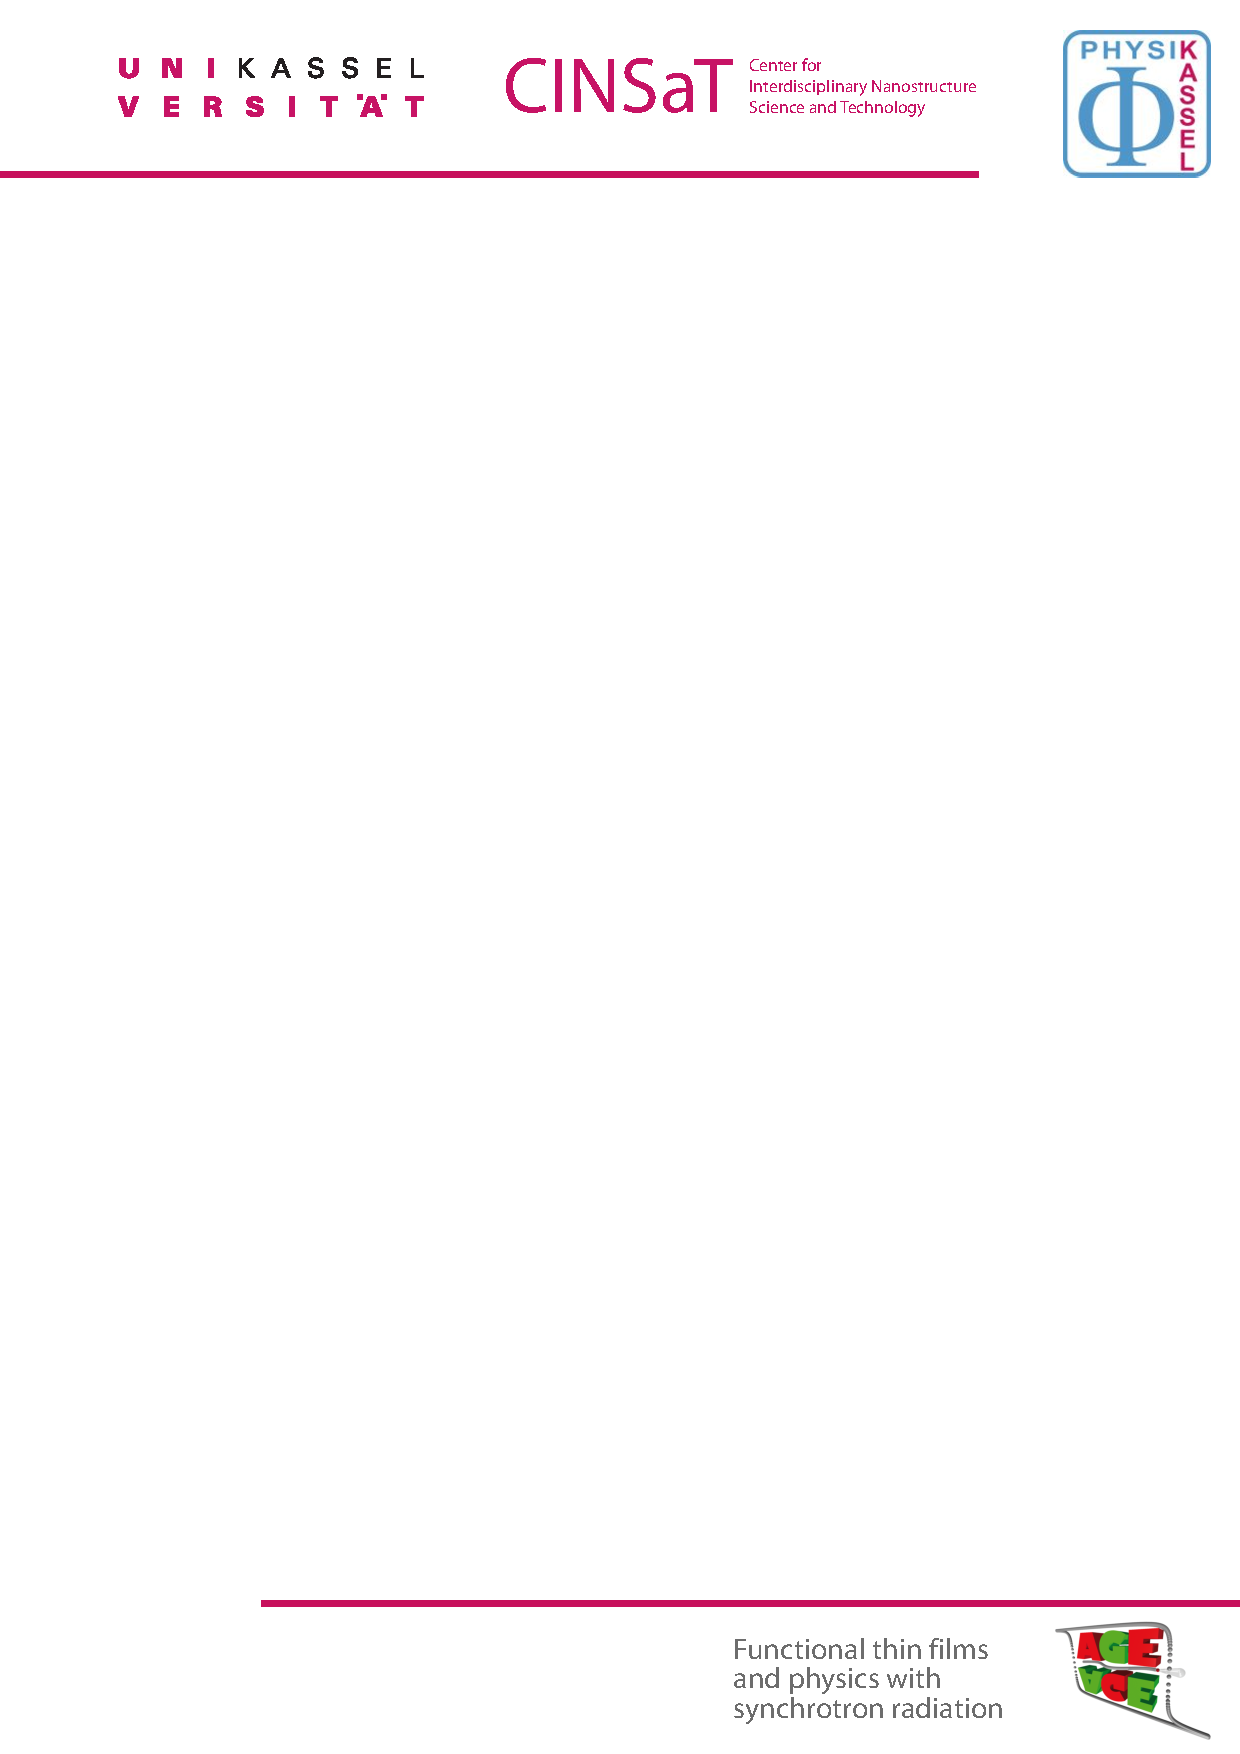
\includegraphics[keepaspectratio]{titlepage/background.pdf}} 

\newgeometry{top=6.5cm,bottom=2.5cm,left=2cm,right=2cm}

\begin{titlepage} 
      \sffamily                                                     
\begin{center}                

{\Large \bfseries                                                                 
  \begin{onehalfspace}                                                           
   Dreidimensionale magnetfeldsequenzen\\[1cm]
  \end{onehalfspace}}                                                               

{\Large
Nikolai Weidt\\[0.5cm]
Kassel, Hoffentlich September 2019 \\[3cm]

{\bfseries Bachelorarbeit im Studiengang Nanostrukturwissenschaften}\\[0.5cm]       
Universität Kassel\\                                                                       
Institut für Physik\\                                                  
Experimentalphysik IV\\[1cm]}                                                                                                                                         
                                                                                          
\end{center}

\vfill

{\large                                                                                                                                                         
\begin{tabbing}
	\textbf{Erstgutachter:} \hspace{1cm} \= Prof. Dr. Arno Ehresmann \\
	\textbf{Zweitgutachter:} \> vlt. Giesen\\
\end{tabbing}}                                                 

\end{titlepage}    

\restoregeometry
 
\SetBgScale{1}
\SetBgAngle{0}
\SetBgOpacity{0}
\SetBgColor{white}
\SetBgContents{}      
